\documentclass[11pt]{article}
%\documentclass[12pt]{article}
%\documentclass[12pt]{article}
%\documentclass[12pt,a4paper]{article}

\usepackage[percent]{overpic}
\usepackage{float}
\usepackage{pgfplots}
%\usepackage[cmbold]{mathtime}
%\usepackage{mt11p}
\usepackage{placeins}
\usepackage{amsmath}
\usepackage{amsthm}
\usepackage{color}
\usepackage{amssymb}
\usepackage{mathtools}
\usepackage{subfigure}
\usepackage{multirow}
\usepackage{epsfig}
\usepackage{listings}
\usepackage{enumitem}
\usepackage{rotating,tabularx}
%\usepackage[graphicx]{realboxes}
\usepackage{graphicx}
\usepackage{graphics}
\usepackage{epstopdf}
\usepackage{longtable}
\usepackage[pdftex]{hyperref}
%\usepackage{breakurl}
\usepackage{epigraph}
\usepackage{xspace}
\usepackage{amsfonts}
\usepackage{eurosym}
\usepackage{ulem}
\usepackage{footmisc}
\usepackage{comment}
\usepackage{setspace}
\usepackage{geometry}
\usepackage{caption}
\usepackage{pdflscape}
\usepackage{array}
\usepackage[round]{natbib}
\usepackage{booktabs}
\usepackage{dcolumn}
\usepackage{mathrsfs}
%\usepackage[justification=centering]{caption}
%\captionsetup[table]{format=plain,labelformat=simple,labelsep=period,singlelinecheck=true}%

%\bibliographystyle{unsrtnat}
\bibliographystyle{aea}
\usepackage{enumitem}
\usepackage{tikz}
\def\checkmark{\tikz\fill[scale=0.4](0,.35) -- (.25,0) -- (1,.7) -- (.25,.15) -- cycle;} 
\newcommand{\xmark}{\ding{55}}%

\usetikzlibrary{decorations.pathreplacing}
%\def\checkmark{\tikz\fill[scale=0.4](0,.35) -- (.25,0) -- (1,.7) -- (.25,.15) -- cycle;}
%\usepackage{tikz}
%\usetikzlibrary{snakes}
%\usetikzlibrary{patterns}

%\draftSpacing{1.5}

\usepackage{xcolor}
\hypersetup{
colorlinks,
linkcolor={blue!50!black},
citecolor={blue!50!black},
urlcolor={blue!50!black}}

%\renewcommand{\familydefault}{\sfdefault}
%\usepackage{helvet}
%\setlength{\parindent}{0.4cm}
%\setlength{\parindent}{2em}
%\setlength{\parskip}{1em}

%\normalem

%\doublespacing
\onehalfspacing
%\singlespacing
%\linespread{1.5}

\newtheorem{theorem}{Theorem}
\newcommand{\bc}{\begin{center}}
\newcommand{\ec}{\end{center}}
\newtheorem{corollary}[theorem]{Corollary}
\newtheorem{proposition}{Proposition}
\newtheorem{definition}{Definition}
\newtheorem{axiom}{Axiom}
\newcommand{\ra}[1]{\renewcommand{\arraystretch}{#1}}

\newcommand{\E}{\mathrm{E}}
\newcommand{\Var}{\mathrm{Var}}
\newcommand{\Corr}{\mathrm{Corr}}
\newcommand{\Cov}{\mathrm{Cov}}

\newcolumntype{d}[1]{D{.}{.}{#1}} % "decimal" column type
\renewcommand{\ast}{{}^{\textstyle *}} % for raised "asterisks"

\newtheorem{hyp}{Hypothesis}
\newtheorem{subhyp}{Hypothesis}[hyp]
\renewcommand{\thesubhyp}{\thehyp\alph{subhyp}}

\newcommand{\red}[1]{{\color{red} #1}}
\newcommand{\blue}[1]{{\color{blue} #1}}

%\newcommand*{\qed}{\hfill\ensuremath{\blacksquare}}%

\newcolumntype{L}[1]{>{\raggedright\let\newline\\arraybackslash\hspace{0pt}}m{#1}}
\newcolumntype{C}[1]{>{\centering\let\newline\\arraybackslash\hspace{0pt}}m{#1}}
\newcolumntype{R}[1]{>{\raggedleft\let\newline\\arraybackslash\hspace{0pt}}m{#1}}

%\geometry{left=1.25in,right=1.25in,top=1.25in,bottom=1.25in}
\geometry{left=1in,right=1in,top=1in,bottom=1in}

\epstopdfsetup{outdir=./}

\newcommand{\elabel}[1]{\label{eq:#1}}
\newcommand{\eref}[1]{Eq.~(\ref{eq:#1})}
\newcommand{\ceref}[2]{(\ref{eq:#1}#2)}
\newcommand{\Eref}[1]{Equation~(\ref{eq:#1})}
\newcommand{\erefs}[2]{Eqs.~(\ref{eq:#1}--\ref{eq:#2})}

\newcommand{\Sref}[1]{Section~\ref{sec:#1}}
\newcommand{\sref}[1]{Sec.~\ref{sec:#1}}

\newcommand{\Pref}[1]{Proposition~\ref{prop:#1}}
\newcommand{\pref}[1]{Prop.~\ref{prop:#1}}
\newcommand{\preflong}[1]{proposition~\ref{prop:#1}}

\newcommand{\Aref}[1]{Axiom~\ref{ax:#1}}
\newcommand{\Dref}[1]{Definition~\ref{def:#1}}

\newcommand{\clabel}[1]{\label{coro:#1}}
\newcommand{\Cref}[1]{Corollary~\ref{coro:#1}}
\newcommand{\cref}[1]{Cor.~\ref{coro:#1}}
\newcommand{\creflong}[1]{corollary~\ref{coro:#1}}

\newcommand{\etal}{{\it et~al.}\xspace}
\newcommand{\ie}{{\it i.e.}\xspace}
\newcommand{\eg}{{\it e.g.}\xspace}
\newcommand{\etc}{{\it etc.}\xspace}
\newcommand{\cf}{{\it c.f.}\xspace}
\newcommand{\ave}[1]{\left\langle#1 \right\rangle}
\newcommand{\person}[1]{{\it \sc #1}}

\newcommand{\AAA}[1]{\red{{\it AA: #1 AA}}}
\newcommand{\YB}[1]{\blue{{\it YB: #1 YB}}}

\newcommand{\flabel}[1]{\label{fig:#1}}
\newcommand{\fref}[1]{Fig.~\ref{fig:#1}}
\newcommand{\Fref}[1]{Figure~\ref{fig:#1}}

\newcommand{\tlabel}[1]{\label{tab:#1}}
\newcommand{\tref}[1]{Tab.~\ref{tab:#1}}
\newcommand{\Tref}[1]{Table~\ref{tab:#1}}

\newcommand{\be}{\begin{equation}}
\newcommand{\ee}{\end{equation}}
\newcommand{\bea}{\begin{eqnarray}}
\newcommand{\eea}{\end{eqnarray}}
\newcommand{\bi}{\begin{itemize}}
\newcommand{\ei}{\end{itemize}}
\newcommand{\Dt}{\Delta t}
\newcommand{\Dx}{\Delta x}
\newcommand{\Epsilon}{\mathcal{E}}
\newcommand{\etau}{\tau^\text{eqm}}
\newcommand{\wtau}{\widetilde{\tau}}
\newcommand{\xN}{\ave{x}_N}
\newcommand{\Sdata}{S^{\text{data}}}
\newcommand{\Smodel}{S^{\text{model}}}
\newcommand{\subhead}[1]{\mbox{}\newline\textbf{#1}\newline}
\setlength{\parindent}{0.0cm}
\setlength{\parskip}{0.4em}
\numberwithin{equation}{section}
\DeclareMathOperator\erf{erf}
%\let\endtitlepage\relax
\begin{document}
\begin{titlepage}
\title{Mixing and Economic Mobility: The Case of Reallocating Geometric Brownian Motion}
\author{Viktor Stojkoski\footnote{Macedonian Academy of Sciences and Arts,~\url{vstojkoski@manu.edu.mk}} \and Alexander Adamou\footnote{London Mathematical Laboratory,~\url{a.adamou@lml.org.uk}} \and Yonatan Berman\footnote{London Mathematical Laboratory,~\url{y.berman@lml.org.uk}} \and Colm Connaughton\footnote{London Mathematical Laboratory and University of Warwick,~\url{c.p.connaughton@warwick.ac.uk}} \and Ole Peters\footnote{London Mathematical Laboratory and Santa Fe Institute,~\url{o.peters@lml.org.uk}}\,\, \thanks{We thank...}}
%\date{First version: August 26, 2018\,\,\,\,\,\,\,\,\,\,\,\,\,\,\,\,\,\,\,\,\,\,\,\,Last revised: \today}
%\date{}
\date{\today}
\maketitle
%\bc
%\red{Preliminary version, please do not circulate}
%\ec
\begin{abstract}
We introduce mixing, a concept from stochastic processes, as a relevant phenomenon for quantifying the ability of individual incomes or wealths to move across the whole distribution. Mixing measures are inherently connected to the concept of economic mobility and will  infer that there is mobility only when income or wealth follows mixing dynamics. Then, there is also a direct equivalence between mixing measures and the magnitude of the standard measures of economic mobility. On the other hand, the opposite is not true. Hence, measuring mobility using standard measures in a non-mixing system may lead to misleading conclusions about the extent of mobility across the whole distribution. We display the the relationship between mixing and mobility by studying the relaxation time, a measure that satisfies the mixing property, in reallocating geometric Brownian motion -- an established model of wealth in a growing and reallocating economy.
\\

\noindent\textbf{Keywords: mobility, inequality, ergodicity economics}
%\\
%\bigskip
\end{abstract}
\setcounter{page}{0}
\thispagestyle{empty}
%\nopagebreak
\end{titlepage}
\pagebreak \newpage
%\nopagebreak
\section{Introduction}\label{sec:introduction}
% What is mobility?
Economic mobility describes ``dynamic aspects of inequality'' \citep{Shorrocks1978}. It quantifies how wealth (or income\footnote{We focus on wealth in this paper, but our findings also apply to income.}) ranks of individuals change over time. Intuitively, when mobility is high, ranks evolve quickly, and the chances of an individual to change her position in the wealth distribution over a given time period are high. When mobility is low, individuals are unlikely to change their rank in the distribution over time, or that it changes slowly.

% How is mobility typically measured?
Mobility measures are assumed to be derived from the joint distribution of wealth at two points in time. On this basis, \citet{Shorrocks1978} described several required properties for the statistical measures of mobility and set the standard for such measures. The author suggested that mobility measures should be normalized, monotonic and independent of the observation period. Any measure defined in a such manner will, however, represent an aggregated value for the extent of mobility within the economy. Therefore, in certain circumstances mobility measures may fail to describe the feasibility of the typical individual to change their wealth rankings.

% This paper
%\YB{In what sense mixing is a property of a mobility measure? I think this should be restated. Mobility and mixing are properties of the process.} \textcolor{red}{I agree, we will rewrite this so as we distinguish mixing and mobility. Do we need to }

As a means do address this issue, this paper defines the concept of \textit{mixing}. Any measure that accounts for this concept will evaluate the ability of \textit{every} individual in an economy to move across the whole steady-state wealth distribution. Thus, it is significantly different from mobility measures, where any change in the rankings is interpreted as existence of mobility. We thereby discuss the impact of mixing on mobility by studying a measure that accounts for this phenomenon. We call this measure the \textit{relaxation time} and interestingly, a variant of it appeared for the first time in the economic mobility literature in Shorocks's seminal paper. Formally, the relaxation time is a feature of stochastic processes that evaluates the convergence of the wealth dynamics of the typical individuals in the economy towards the steady state distribution. When wealth is a mixing observable \citep{PetersAdamou2018c}, if the wealths of an arbitrary group of individuals is followed over time, the distribution of wealth within this group will gradually become similar to the steady-state wealth distribution. The characteristic time of this convergence process is the relaxation time. Put simply, it is the time scale over which individuals mix into the wealth distribution. When mixing is rapid, \ie the relaxation time is short relative to the window of observation, we could interpret that as high wealth mobility. Slow mixing is interpreted as low mobility.

% We study RGBM
We then consider Reallocating Geometric Brownian Motion (RGBM \citep{MarsiliMaslovZhang1998,LiuSerota2017,BermanPetersAdamou2019}) as a model for wealth dynamics and study mixing in this model. In RGBM, individual wealth undergoes random multiplicative growth, modeled as Geometric Brownian Motion (GBM), and is reallocated among individuals by a simple pooling and sharing mechanism. RGBM is a null model of an exponentially growing economy with social structure. It has three parameters representing economic growth, random shocks to individual wealth, and economic interaction among agents, quantified by a reallocation rate. This model is known to reproduce several important stylized facts. In particular, when the reallocation is from the rich to the poor, the rescaled wealth distribution converges to a stationary distribution with a Pareto tail. The model has both ergodic and non-ergodic regimes, characterized by the sign of the reallocation rate parameter \citep{BermanPetersAdamou2019}.

% What is the mixing time in RGBM?
We find that in the mixing regime of RGBM, the relaxation time scales with the inverse of the reallocation rate. As the reallocation rate becomes higher, \ie when a larger share of each individual's wealth is pooled and then shared per unit time, the relaxation time becomes shorter proportionally, and mobility increases. As the reallocation rate approaches zero, relaxation times get longer, and mobility lower. In RGBM, decreasing reallocation rates also lead to increasing inequality. Hence, this result is in line with the empirical observation that as inequality increases mobility decreases, and vice versa \citep{corak2013}. %There is also a direct relationship between mixing time and standard measures of economic mobility. The intragenerational copulas produced by RGBM closely resemble Gumbel copulas \citep{Gumbel1958,TrivediZimmer2007}, often used in the mobility literature.

% Mixing in non-ergodic systems
In practice, however, many economic systems are best modeled as non-ergodic, and hence non-mixing \citep{Peters2019b}. In particular, \citet{BermanPetersAdamou2019} argue that the US economy is best described in RGBM as one in which wealth is systematically reallocated from poorer to richer, \ie the reallocation rate is negative. In this case, even though the standard measures of economic mobility might suggest existence of mobility, there is no mixing. Thus, measuring mobility using standard measures under this regime may lead to misleading conclusions that everyone is able to move across the wealth distribution. The thorough study of RGBM in this regime is outside of the scope of this paper and left for future work.

% Plan
The paper is organized as follows. In~\Sref{mixing-time} we mathematically define mixing and compare its characteristics to those of standard mobility measures. In the same section, we introduce the relaxation time as a measure that evaluates the degree of mixing in an economy. \Sref{rgbm} relates mobility and mixing in reallocating geometric Brownian motion as a model for wealth. We discuss our findings in~\Sref{discussion}.

\section{Mixing and mobility}
\label{sec:mixing-time}

\subsection{Definition}
%\YB{I would first give an intuitive definition and only then a mathematically precise definition, also in a more standard mathematical structure: let $x$ be, etc.}


The concept of mixing comes from probability theory and statistical physics. In physical terms, it describes the property of a dynamical system being strongly intertwined. That is, in any set of particles in a dynamical system, the fraction of the particles found within a particular region in the \textit{phase space} (the space of the variable $x$ characterizing the particles, wealth in our case), is proportional to the volume of that region in the phase space. Figuratively, we can think of an economy as a cup of coffee and of some person's wealth as milk poured in the coffee. If the system is mixing, then the milk will spread across the coffee over time  and eventually it will be spread equally.
 
Mathematically we define mixing as follows. Let $x_i(t)$ denote the wealth at time $t$ of the $i$-th individual in a population of size $N$. Moreover, let $P(x,t)$ be the probability density function that describes the distribution of wealth in the population at the same time point. If the economy is mixing, then starting from an initial point in time $t = 0$ in which every individual in the population has \textit{identical} wealth $x_i(0) = x_0$, then $P(x,t)$ will in each subsequent time point resemble more and more a predefined target steady state distribution $P^*(x,t)$, and it will eventually converge to it. A standard way for evaluating this characteristic is through the $\beta$-mixing coefficient. This coefficient measures the total variational distance between the wealth distribution in time $t$ and the steady state distribution, i.e.,
\begin{align*}
    \beta(t) &= || P(x,t) - P^*(x) ||,
\end{align*}
where $||g(y)|| = \int |g(y)| dy$ is the $L^1$ norm of $g$. The wealth dynamics is said to be $\beta$-mixing if $\lim_{t \to\infty} \beta(t) = 0$ (See for more details \citep{drees2000weighted}). %Any measure that is derived from the properties of $\beta(t)$ satisfies the mixing property.

In economic terms, mixing implies that the system does not discriminate individuals on the basis of their history: it is possible for everyone to move between any ranks in the distribution over time. Thus this concept can be seen as a mathematical manifestation of the ``American Dream''. 

This is naturally linked to economic mobility, as defined by standard measures of mobility, however the two are not the always the same. As we will see in~\Sref{measures}, there is always a relationship between measures that incorporate mixing and standard mobility measures, whenever mixing exists in the system. However, the standard measures may still indicate that there is some level of mobility even when mixing does not occur. Yet, the existence of such mobility, a degree of which always exists practically, does not guarantee mixing as this observation depends on the existence of mobility between \textit{every} quantile in the wealth distribution\footnote{This idea was already described by \citet{Mcfarland1970}.}.
 
We hereby emphasize that mixing is strongly related to the concept of ergodicity. However, the latter is a broader concept: An observable $x$ is said to be ergodic if its time-average is to its ensemble averages at any given time. Put differently, ergodicity implies that every trajectory moves around the phase space over time according to the steady state distribution of $x$. Hence, every dynamical system that is mixing is also ergodic, but the opposite is not necessarily true.

\subsection{Implications of mixing to measures of mobility}

To understand the differences between measures that quantify the extent of mixing and the information produced by standard measures of mobility here we describe their similarities and differences. For this comparison we utilize two standard measures of economic mobility: Spearman's rank correlation and the intragenerational earnings elasticity (IGE)\footnote{In fact, the rank correlation and the IGE are both measures of immobility, and to consider them as measures of mobility one has to consider their complement or their inverse.}. These measures describe attributes of the bivariate joint wealth distribution at two points in time. Such distributions are usually modeled via copulas. Mathematically, a copula can be represented by a simple model in which the wealth transition matrix is parametrized\footnote{One might argue that mixing as a concept is equivalent to the notion of \textit{irreducibility} in transition matrices. However, transition matrices already aggregate the wealth dynamics into quantiles and thus may distort the picture of the extent of mobility.}. A widely used model is the Gumbel copula. It is able to reproduce realistic wealth-rank transition matrices, representing higher mobility at the bottom of the distribution than at the top \citep{JanttiJenkins2015}. The Gumbel copula is uniquely defined by a single parameter $\theta$: a larger dependence implies less mobility. Due to its direct relationship with economic mobility, we also include this parameter in the comparative analysis. Technical background for the standard mobility measures is given in Appendix~\ref{sec:standard-mobility-measures}.

To elucidate the differences and similarities, we consider five properties that a mobility measure may have and use them to characterize mobility measures. First, following \citet{Shorrocks1978} we identify the properties of 1) \textit{normalization} -- the values that the mobility measure may take are bounded in a closed interval; 2) \textit{monotonicity} -- if a new structure is imposed in the wealth dynamics of some individuals then this is reflected in the value of the measure, and 3) \textit{period dependence} -- the mobility predicted by the measure is dependent on the temporal difference $\delta$ between the periods that are used for its estimation. In addition, we follow \citet{cowell2018measuring}, and add to our analysis the property of 4) \textit{distribution dependence} -- whether the mobility predicted by the measure is dependent on the shape of the empirical wealth distributions that are used for its estimation or not. %Lastly, we introduce the property of 5) \textit{mixing} which, as argued above, quantifies whether the mobility measure accounts for the feasibility of moving across the whole wealth distribution, \ie if all individuals are able to change their wealth status.

Table~\ref{tab:mobility-properties} details the properties that are satisfied by the standard mobility measures which we study. For comparison, the table also gives the properties that are typically captured by measures that quantify mixing, when they are used to evaluate the mobility within an economy. % (\YB{again, unclear what this means})
We see that mixing measures may not satisfy the normalization property. Also, the IGE does not satisfy this property. However, we state that normalization is just a standard procedure that can be implemented to any measure, and measures that account for mixing can be easily adjusted to satisfy this property (\YB{How?}) \textcolor{red}{VS: this can be done in various ways. For example our measure, the relaxation times, can be put in a value between 0 and 1 by writing it as $e^{-1/\texttt{relaxation times}}$. This measure was actually defined by Shorrocks in terms of transition matrices (when we look at transition matrices then the relaxation time is the second eigenvalue, exactly as in our case. Other approaches can also be used such as implementing a logit transform etc.}

\begin{table}[h]
\caption{\textbf{Properties of mobility measures.\label{tab:mobility-properties}}}
\resizebox{\textwidth}{!}{%
\begin{tabular}{l||ccccc}
\textbf{Measure }  & \multicolumn{4}{c}{\textbf{Property}} \\\hline
           & Normalization & Monotonicity & P. dependence & D. dependence \\\hline
Mixing measures         & ?             & $\times$            & $\times$                 & \checkmark           \\
Spearman Correlation & \checkmark             & \checkmark            & \checkmark                 &  $\times$                         \\
IGE                  & $\times$             & \checkmark            & \checkmark                 & \checkmark                           \\
Gumbel parameter     & \checkmark             & \checkmark            & \checkmark                 & $\times$   \\                
\end{tabular}}
\end{table}

More importantly, measures for mixing will not satisfy the monotonicity and the period dependence properties. The inability to satisfy the monotonicity property appears because monotonicity implies that if there is mobility between certain quantiles of the wealth distribution, it will be translated with existence of mobility in the standard measures. The three described measures represent aggregated values of the changes in the wealth rankings of the individuals which constitute the population between two time periods $t$ and $t+\delta$. Thus, if the transition matrix is slightly perturbed between the two periods, it will result in change in the magnitude of mobility predicted by the measure. Measures for mixing, on the other hand, are not monotonic unless there is already mobility between every quantile. In every other case they will imply zero mobility.

Next, we study the distribution dependence property, a phenomenon captured by mixing measures. From the three standard measures, only the IGE is dependent on the shape of the wealth distributions that are used for its estimation, whereas the other two measures are not. This dependence indicates that measures for mixing will not be interpreted similarly when the underlying wealth distribution remains unchanged, and when it becomes more and more unequal.

%Lastly, let us look at the mixing property, which is evidently not featured in the studied standard measures. In this context, we again emphasize that this property states that the extent of mobility predicted by the measure will be dependent by the feasibility of \textit{all} individuals to change their wealth rankings. Measures that incorporate this property quantify the mobility of the typical representative of the population and, hence, do not represent an aggregated value.


\subsection{An example for a mixing measure}
\label{sec:relaxation-time}
As an example for a measure that quantifies the degree of mixing, we consider the inverse of the rate of convergence $r$ towards the steady state distribution $P^*(y)$ of the transformation of wealth $y$, i.e.,
%
\be
    r = - \lim_{t \to \infty} \frac{1}{t} \log \beta(t).
\ee
%
%\YB{Explain where this comes from.} \textcolor{red}{We explain how it is derived further down in the RGBM example. Do you think that some parts of it are better to be put here? Please see the part in red in Sec. 3.2.}
This measure is also known as the \textit{relaxation time} towards the steady state distribution. It provides a characteristic time scale over which individuals mix into the wealth distribution. In the coffee example analogy, the relaxation time would quantify the time required for the milk to blend with the coffee. This enables the measure to be used for appropriate comparison between different time periods and economies. Notice that the relaxation time does not satisfy the normalization property of mobility measures. We purposely refrain from this procedure because emphasize whether some value of relaxation time is high or low, as compared to other economies. Strictly speaking, using time units allows us say that when mixing is rapid, \ie the relaxation time is short relative to a relevant window of observation, then there is high wealth mobility. Slow relaxation times is interpreted as low mobility. A similar measure, based on wealth transition matrices that satisfies the normalization properties, was studied in \citep{Shorrocks1978}.

The estimation of the relaxation time in a system in which the process governing the wealth dynamics is known, can be done easily by studying the spectral properties of the process (See~\Sref{relax-time-rgbm}). Its estimation in empirical situations when the wealth dynamics is unknown, though, is a little bit more complicated. To illustrate this, let us first present an empirical procedure for estimating the relaxation times. The described properties of a mixing economy can be utilized in this context. The first step is defining a relevant steady state distribution to which the rescaled transformation of wealth converges. We then select a subsample of size $K$ consisting of the individuals that are closest to the mean wealth (\ie the typical individuals in the economy), track the subsample wealth distribution over time and quantify the difference between the subsample wealth distribution and the steady state distribution with the total variational distance. Notice that, when the relaxation time is estimated using this procedure, one uses an estimate for the wealth distribution based on an empirical histogram. It is widely known that histograms can only resemble the theoretical distribution only to a certain extent because they are constituted of a finite sample size. Therefore, in a mixing economy the total variational distance will exhibit two states. First, there will be a relaxation time state during which the two distributions will converge towards each other, and the distance will decrease. After a transitory phase, there will be a stable state. In the stable state the log of the distance reaches a plateau and fluctuates around this plateau. The magnitude of the plateau will be determined by the subsample size: smaller sample sizes will exhibit higher plateau and vice versa. This is a finite sample size effect. In a mixing economy, the total variational distance will be small and exhibit statistical significance in the stable state. Moreover, the point at which the plateau is reached will in general be higher than the mixing time. Hence, one can use the time point at which the total variational distance becomes significant as an upper bound for the relaxation time and as a sign that the economy is mixing. Interestingly, this exact procedure is used in Markov Chain Monte Carlo to track the convergence to the steady state and is called the ``mixing time''.
%\YB{Why the KS statistic? I think it is a bit confusing now. Can't it be done more generally following the definition in section 2.1? }\textcolor{red}{VS: I think that it can be done. I just am not sure... will need to study this...}

\Fref{mixing-time} summarizes the procedure in a fictive example. The blue line is the log of the total variational distance as a function of time. The dashed black line is the slope of the relationship between the statistic and time during the two different states. The inset plots provide snapshots for the wealth distribution of the subsample (i.e., estimates based on a histogram) at different time points (red dashed lines). For comparison, the snapshots also include the form of the selected steady state distribution (black line). Notice that initially, at $t_1$, the subsample distribution is very narrow and does not resemble the steady state distribution. The wealths in the subsample evolve, and in $t_2$ and $t_3$ the subsample distribution becomes closer to the steady state distribution. Eventually, the subsample distribution resembles the steady state distribution. The upper bound for the relaxation time is the point at which the total variational distance becomes statistically significant. 

\begin{figure}[!htb]
\centering
\includegraphics[width=1.0\textwidth]{figs/fig_mixing_time.pdf}
\caption{\textbf{Quantifying relaxation times in an empirical system.} The blue line shows the log of the statistical distance between the subsample and the target wealth distribution. The black dashed line is the slope of the line which describes the relationship between the log of the statistical distance and time, estimated separately for the relaxation period and the sable state period. The inset plots give snapshots for the empirical form of subsample distribution (red dashed line) and the target distribution at different points in time $t_1 < t_2 < t_3 < t_4$. We stress out that in a non-mixing economy, the KS statistic will either converge to a fixed value but it will remain statistically insignificant or it will be a divergent quantity. In Appendix~\ref{sec:rgbm-numerical-mixing-time} we present an example for the implementation of the procedure in the RGBM model.
\label{fig:mixing-time}}
\end{figure}
\FloatBarrier







 %Nonetheless, as we will see later on, we purposely refrain from this procedure when we will define our measure that has the mixing property because in that case it will be impossible to tell whether some value of mixing time is high or low, unless it is compared to other economies. Instead, using time units allows us say that when mixing is rapid, \ie the mixing time is short relative to a relevant window of observation, then there is high wealth mobility. Slow mixing is interpreted as low mobility. % This overcomes the necessity to define high or low mobility with respect to other countries or to the past.






%Using mixing times overcomes the limitations of the standard measures in several ways. First, the mixing time is measured in units of time. This means that when mixing is rapid, \ie the mixing time is short relative to a relevant window of observation, we could interpret that as high wealth mobility. Slow mixing is interpreted as low mobility. This overcomes the necessity to define high or low mobility with respect to other countries or to the past. Second, the mixing time is a finite quantity only when each individual is able to move across the whole distribution of wealth. Therefore, it does not represent an aggregate measure of the mobility in the economy. It captures the feasibility of \textit{all} individuals to change their wealth status.





\section{Mixing in a simple model of an economy}\label{sec:rgbm}
\subsection{Reallocating geometric Brownian motion}

To illustrate the application of mixing in economic systems, we use Reallocating geometric Brownian motion (RGBM), a simple model for wealth dynamics \citep{BermanPetersAdamou2019}. Under RGBM, wealth is assumed to grow multiplicatively and randomly, in addition to a simple reallocation mechanism. The dynamics of the wealth of person $i$ are specified as
%
\be
\mathrm{d} x_i = x_i \left( \mu \mathrm{d}t + \sigma \mathrm{d}W_i \right) - \tau \left( x_i - \langle x \rangle_N \right) \mathrm{d}t\,,
\label{eq:rgbm}
\ee
%
with $\mu > 0$ being the drift term, $\sigma > 0$ the fluctuations amplitude, and $\mathrm{d}W_i$ is an independent Wiener increment, $W_i(t) =\int_0^t \mathrm{d}W_i$. $\tau$ is a parameter that quantifies the reallocation of wealth. It implies that every time period $\mathrm{d}t$, everyone in the economy contributes a fraction $\tau\mathrm{d}t$ of their wealth to a central pool. The pool is then shared equally across the population ($\langle x \rangle_N$ is per-capita wealth). This parameter encapsulates multiple effects, \eg collective investment in infrastructure, education, social programs, taxation, rents paid, or private profits.

Under RGBM, the average wealth in a large population grows like $e^{\mu t}$. Rescaling by $e^{\mu t}$, the dynamic behavior of RGBM is strictly dependent on the relation between $\tau$ and $\sigma$, and the rescaled wealth can be both mixing and non-mixing. In RGBM, rescaled wealth is mixing when $\tau > 0$
and the model exhibits mean-reversion as each $x_i$ reverts to the population average $\langle x \rangle_N$. The dynamics of the rescaled wealth $y_i = x_i / \langle x \rangle_N$ can be described as
%
\be
    \mathrm{d} y =   y \sigma  \mathrm{d} W - \tau (y - 1)  \mathrm{d}t\,,
    \label{eq:rescaled-rgbm}
\ee
%
and its stationary distribution is (see \citep{BermanPetersAdamou2019})
%
\be
P^*(y) = \frac{(\zeta - 1)^{\beta}}{\Gamma(\zeta)} \exp{\big(-\frac{\zeta - 1}{y}\big)} y^{-(1+\zeta)}\,,
\label{eq:rgbm-stationary-distribution}
\ee
%
where $\zeta = 1 + \frac{2 \tau}{\sigma^2}$ and $\Gamma(\cdot)$ is the Gamma function. The distribution has a power-law tail. The exponent of the power law, $\zeta$, is called the Pareto tail parameter, and can be used as a measure of economic equality \citep{Cowell2011}. More importantly, important stylized facts are recovered: the larger $\sigma$ (more randomness in the dynamics) and the smaller $\tau$ (less reallocation), the smaller the tail index and the fatter the tail of the distribution, leading to higher inequality.

\subsection{Relaxation time in RGBM}
\label{sec:relax-time-rgbm}
The estimation of relaxation time in a stochastic process is usually done by investigating the Fokker-Planck equation which describes the evolution of the probability density function. In RGBM this equation reads
\begin{align}
       \frac{\partial}{\partial t}P(y,t)= \tau \frac{\partial}{\partial x} \left[(y-1) P(y,t)\right] + \frac{\sigma^2}{2}\frac{\partial^2}{\partial x^2} \left[ y^2 P(y,t) \right].
\end{align}
The equation is an appropriate generalization of a transition matrix for a discrete space process to processes with continuum of states. Hence, the analysis follows exactly in the same manner: the critical statistic of the Fokker-Planck equation that governs the convergence of $P(y,t)$ to $P^*(y)$ is the largest nontrivial eigenvalue of the corresponding Fokker-Planck operator, that is, the second largest eigenvalue. In a mixing system the largest eigenvalue will be zero, whereas the second $\lambda_2$ will be \textit{negative}, and $\beta(t) \propto e^{\lambda_2 t}$. We refer to~\cite{gabaix2016dynamics} for a detailed mathematical background on estimating the relaxation time in wealth/income dynamics. 

An extensive study for the eigenvalues of RGBM was done by~\cite{LiuSerota2017}. The authors showed that the second largest eigenvalue is simply $-\tau$, and therefore the relaxation time will exist only when $\tau > 0$ and it will be equal to $1/\tau$. The interpretation behind this result is fairly intuitive -- in an economy in which reallocation from the rich to the poor is stronger, mixing is faster. On the other hand, as the reallocation rate approaches zero, relaxation times get longer, and mobility, as defined by the concept of mixing lower. When the reallocation rate reaches the point $0$ and for values lower, there is no stationary distribution to which rescaled wealth converges, and thus there is no possibility for mixing in the economy. Then, the relaxation time will be infinite. We point out that while $\tau <0$ implies no mixing, that does not mean that the standard mobility measures will also indicate no mobility. In fact, for any positive fluctuation amplitude $\sigma$ there will be randomness in the system. This randomness may drive changes in the observed wealth rankings, and as a result the standard measures may display a certain degree of mobility.

%The mixing time in RGBM can also be estimated using the estimation procedure described above. If a subsample of the population is considered, its distribution will converge to the steady state distribution of the whole population (when $\tau > 0$). The reciprocal of the convergence rate is the mixing time (see \fref{mixing-time}), and will also be equal to $1/\tau$.

\subsection{Mixing and standard measures of mobility}\label{sec:measures}

In RGBM, unlike the relaxation time, standard measures of mobility depend on the fluctuation amplitude $\sigma$, and not only on $\tau$. This is a consequence of the randomness playing a significant role in the wealth dynamics when we consider time frames that are shorter than the time required for the system to relax. In what follows we describe the relationship between relaxation time and the standard measures of mobility in RGBM.

\paragraph{Spearman's rank correlation:} Spearman's rank correlation is inversely related to the relaxation time in RGBM. The rank correlation is also dependent on the fluctuation amplitude $\sigma$ and the temporal difference $\delta$ between the two periods that are being compared. Larger values for both parameters lead to greater economic mobility. This can be seen in~\fref{rgbm-standard-measures}A, where we plot the log of the rank correlation divided by $\delta$ as a function of $\tau$ for various noise amplitudes.

\begin{figure}[!htb]
\centering
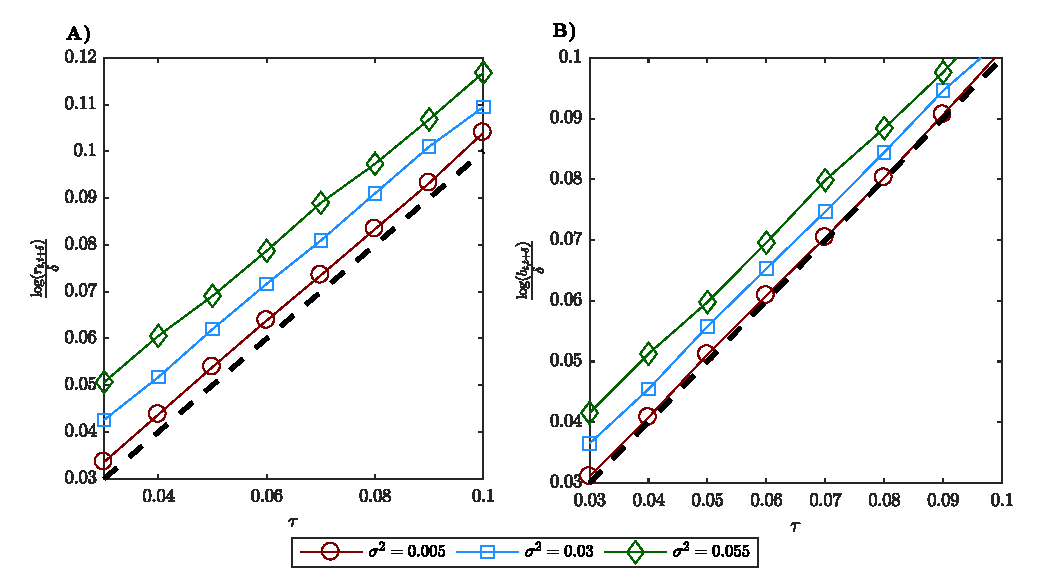
\includegraphics[width=1.0\textwidth]{figs/fig_rgbm_standard_measures.eps}
\caption{\textbf{Relaxation time and standard measures of economic mobility.} \textbf{A)} Log of the Spearman's rank correlation divided by the temporal difference as a function of $\tau$. \textbf{B)} Same as \textbf{A)}, only on the y axis is the log of the IGE. \textbf{A-B} The dashed black line has a slope 1. The simulations used $\delta = 20$ years and $N = 10^4$ people.
\label{fig:rgbm-standard-measures}}
\end{figure}

\paragraph{Intragenerational earnings elasticity:} Similarly to the properties of the rank correlation, and as depicted in~\fref{rgbm-standard-measures}B, the IGE depends on both the fluctuation amplitude and the magnitude of reallocation.

\paragraph{Transition matrices:} As evidenced in~\fref{rgbm-wealth-matrices}A, the transition matrices in RGBM reproduce the asymmetric property of the real world transition matrices and are well-approximated by the Gumbel copula (\fref{rgbm-wealth-matrices}B). In \fref{rgbm-wealth-matrices}C we visualize the relationship between Gumbel parameter $\theta$ and the reallocation parameter $\tau$ for various fluctuation amplitudes. We find that there is an inverse relationship between $\theta$ and $\tau$, and the Gumbel parameter slope is further determined by the magnitude of $\sigma$. As $\tau$ increases, the value of the $\theta$ decreases, though disproportionately. We hereby point out that the $\theta$ parameter and the rank correlation share a direct relationship which cannot be analytically represented. As a way to visualize this relationship in \fref{rgbm-wealth-matrices}D we plot the rank correlation as a function of $\tau$.

\begin{figure}[!htb]
\centering
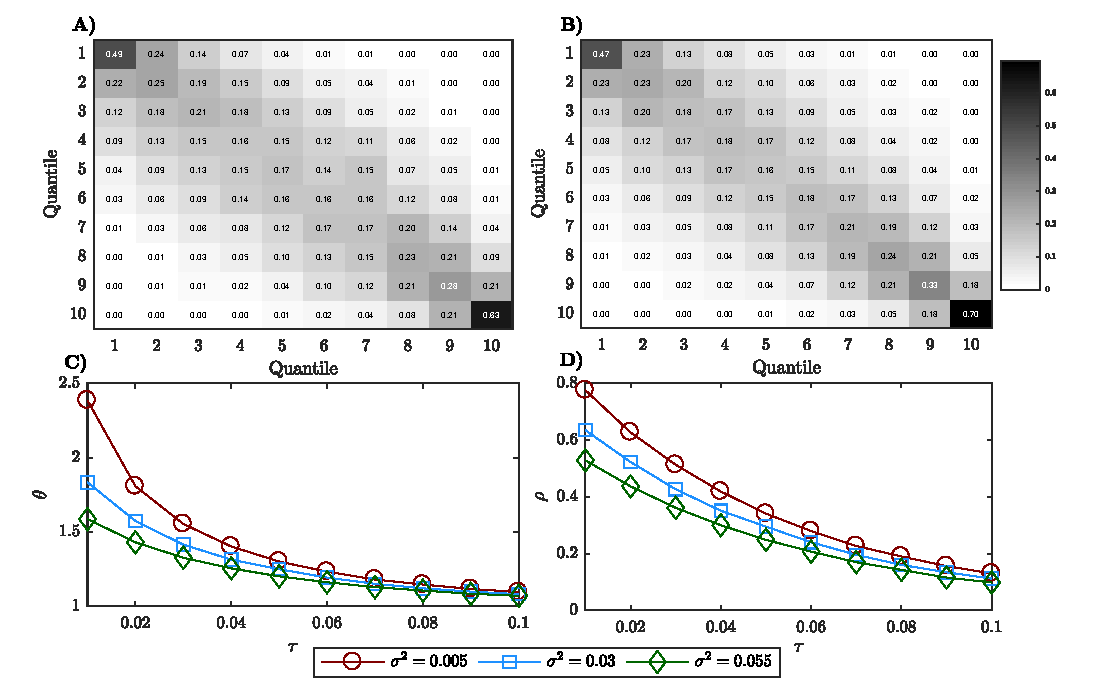
\includegraphics[width=1.0\textwidth]{figs/fig_rgbm_gumbel_v2.eps}
\caption{\textbf{Relaxation time and wealth transition matrices.} \textbf{A)} Transition matrix for the stationary regime of RGBM estimated with $\tau = 0.02$ per year, $\sigma^2 = 0.01$ per year and $N = 10^4$ people. \textbf{B)} An example for a transition matrix from data simulated from a Gumbel copula whose parameter $\theta$ is chosen to be in accordance with the RGBM parameters used in \textbf{A)}. \textbf{C)} The relationship between the Gumbel copula parameter $\theta$ and the reallocation parameter $\tau$ in the stable state of RGBM. \textbf{D)} The relationship between the Gumbel copula parameter $\theta$ and the rank correlation $\rho$ in the stable state of RGBM. The parameters were estimated from a transition matrix in which $\delta = 20$ years and $N = 10^4$ people.
\label{fig:rgbm-wealth-matrices}}
\end{figure}
\FloatBarrier

\subsection{The Great Gatsby curve in RGBM}

Quantifying mobility in RGBM using relaxation times allows us to study the relationship between mobility and inequality. A convenient illustration of this relationship is the Great Gatsby curve, which describes an association between inequality and the intergenerational earnings elasticity across countries \citep{krueger2012,corak2013}, showing that economic \textit{immobility} and static inequality are positively related across countries.

As elaborated previously, in RGBM the relaxation time, quantifying immobility, is $1/\tau$. The Pareto tail parameter is $\zeta$, the inverse of which is a measure of inequality. We get that
%
\be
\frac{1}{\tau} = \frac{2}{\sigma^2\left(\zeta - 1\right)}\,.
\ee
%
\fref{rgbm-great-gatsby} displays this relationship, demonstrating that RGBM reproduces the qualitative empirical observation that inequality and immobility are positively related. More importantly, we can use RGBM and the concept of mixing to interpret the nature of the relationship. In particular, in a more unequal (but mixing) system, it takes much more time for an individual to visit every rank in the wealth distribution simply because the distribution is more spread. 

\begin{figure}[!htb]
\centering
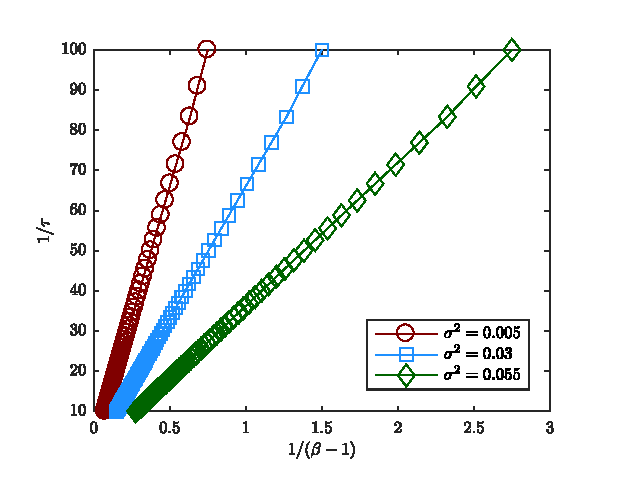
\includegraphics[width=10cm]{figs/fig_great_gatsby.eps}
\caption{\textbf{The Great Gatsby curve in RGBM.} Relaxation time as a function of the inverse of the Pareto Tail coefficient in RGBM. The line colors correspond to the magnitude of the noise amplitude. 
\label{fig:rgbm-great-gatsby}}
\end{figure}

\FloatBarrier

\section{Discussion} \label{sec:discussion}

The existence of mobility between every rank within an economy is postulated on mixing wealth dynamics. Standard mobility measures may fail to account for this property, whereas measures that capture the mixing property overcome the aforementioned issues. As we showed, with the relaxation time example, every mobility measure that also quantifies mixing will not be monotonic, and this particular characteristic allows them to quantify whether the system is in a mixing state or not. Whenever the system is not mixing, measures of mixing will suggest no mobility. This is because mixing is predicated on the existence of an ergodic transformation of wealth which exists only in a certain case. In particular, the ergodic transformation is characterized with a steady-state distribution and the transformed wealth distribution of any arbitrary subset of individuals belonging to the population will gradually become similar to it, if followed for long enough.

Studies of wealth inequality often make the hypothesis that the mixing transformation is given by the rescaled wealth. This case was also discussed here. However, a growing body of evidence suggests that in reality rescaled wealth might also be a non-ergodic, and hence non-mixing observable. For instance, \citet{BermanPetersAdamou2019} found that, in the case of RGBM wealth dynamics, negative reallocation ($\tau < 0$) prevails in the US economy. Then, measures such as the relaxation time are undefined and mobility across the whole distribution is non-existent.
%Even in times when the reallocation was positive, the mixing time was low (between 50 and 100 years).
 
Nevertheless, another transformation of wealth might exist which is mixing, and measures in terms of it might suggest that there is mixing in the economy. Then mobility between every quantile exists, but can be defined in terms of an another concept.  For example, mobility can be defined in terms of growth of wealth or in terms of reduction of the unpredictability of wealth dynamics. Different concepts also require different analysis approaches, as they illuminate distinct extent to which mobility is socially desirable. In other words, depending on the definition of economic mobility, an increase in economic mobility will not always translate into increased economic welfare. Hence, discovering the relevant wealth transformation is extremely important for policymakers to produce adequate measures for optimizing the mobility within an economy. We refer to \citet{JanttiJenkins2015} for a lengthy discussion on the various concepts of economic mobility and their social implications.

We conclude with some notes on the empirical implementation of the relaxation time as a measure of mixing. As elaborated in the previous sections, there are two strategies that can be used to evaluate empirically the relaxation time in an economy. The first one is by using the procedure described in~\Sref{relaxation-time}. The main advantage of the procedure is that it offers a non-parametric approach for estimation of a upper bound for the relaxation time which is independent on the assumption of wealth dynamics. However, this is an expensive procedure to perform in reality as it requires a detailed track for the wealth of a particular set of individuals. This will be even more pronounced if the convergence time to the steady state distribution is slow. The second strategy requires an assumption for the wealth dynamics of each individual in the population. By combining this assumption with data on the properties of the observed wealth distribution, various methods can be implemented to infer the parameters which govern the wealth dynamics. Once the parameters are inferred, the relaxation time can be easily estimated via the spectral properties of the wealth dynamics. While the presented method offers an inexpensive way for quantifying relaxation time, it is highly stylized in the sense that it is necessary to first assume wealth dynamics. Nonetheless, in the absence of simpler procedures, the second strategy acts as the starting point for the development of a more comprehensive methodology for estimating the mixing properties of an economic system. We believe that with the rapid development of data gathering methods and the improved understanding of wealth dynamics within a population, some of these shortcomings will be overcome, yielding a more in-depth interpretation of mixing in real economies.


%\bibliography{../LML_bibliography/bibliography}
\bibliography{mixing-time}
\clearpage

\appendix

\section{Definitions of standard mobility measures}\label{sec:standard-mobility-measures}

\paragraph{Spearman's rank correlation:} Spearman's rank correlation $\rho_{t_m,t_n}$is defined on a joint distribution of wealth at two points in time, $t_m$ and $t_n$ ($t_m < t_n$). It is defined as
%
\be
    \rho_{t_m,t_n} = 1 - \frac{6\sum_i \left[rg\left(\mathrm{x}_i\left(t_m\right)\right) - rg\left(\mathrm{x}_i\left(t_n\right)\right)\right]^2}{N\left(N^2-1\right)}\,,
\ee
%
where $rg(\mathrm{x})$ is the rank transformation of $\mathrm{x}$, $\mathrm{x}_i(t)$ is the wealth of individual $i$ in period $t$ and $N$ is the population size. This measure is bounded between $-1$ and $1$. $\rho_{t_m,t_n} = 1$ suggests perfect immobility, a state in which there is no change in wealth ranks between the two points in time. Lower values suggest greater economic mobility.

\paragraph{Intragenerational earnings elasticity:} The intragenerational earnings elasticity is defined as the slope $b_{t_m,t_n}$ of the regression
%
\be
   \log\left(\mathrm{x}_i\left(t_n\right)\right) = b_0 + b_{t_m,t_n} \log\left(\mathrm{x}_i\left(t_m\right)\right) + u_i\,,
\ee
%
where $b_0$ is the intercept and $u_i$ is the error term. This is a simple linear regression and therefore,
%
\be
    b_{t_m,t_n} = \mathrm{corr}\left(\log\left(\mathrm{x}\left(t_n\right)\right),\log\left(\mathrm{x}\left(t_m\right)\right)\right) \frac{\mathrm{var}\left(\log\left(\mathrm{x}\left(t_n\right)\right)\right)}{\mathrm{var}\left(\log\left(\mathrm{x}\left(t_m\right)\right)\right)}\,,
    \label{eq:iee-estimation}
\ee
%
where $\mathrm{corr}(\mathrm{x},\mathrm{y})$ is the correlation between the variables $\mathrm{x}$ and $\mathrm{y}$ and $\mathrm{var}(\mathrm{x})$ is the variance of $\mathrm{x}$. As with the rank correlation, lower IGE also indicates greater mobility. However, this measure is unbounded and may take on any real values.

\paragraph{Wealth transition matrix:} The wealth transition matrix disaggregates wealth rankings and summarizes economic mobility in a
transition matrix $\mathbf{A}$ in which the elements $A_{kl}$ quantify the probability that an individual in wealth quantile $k$ in period $t_m$ is found in wealth quantile $l$ in period $t_n$. In a perfectly mobile economy, the entries of the transition matrix are all equal to each other. This would correspond to $0$ rank correlation. In an immobile economy, on the other hand, the largest values are concentrated in the diagonal entries. A perfectly immobile case, of rank correlation $1$, would correspond to the identity transition matrix.

\section{Numerical estimation of Relaxation times in RGBM}\label{sec:rgbm-numerical-mixing-time}

We use RGBM to numerically present the procedure described in~\Sref{mixing-time}. In the concrete example, we focus on the role of the subsample size, $\tau$ and $\sigma$ in the duration of the relaxation period and the estimation of the relaxation time measure. 

For this purpose, in~\Fref{rgbm-mixing-time}A-B we plot the the total variational distance (on a log scale)  as a function time and vary the subsample size, reallocation rate and the noise amplitude. Intuitively, the reallocation rate uniquely determines the relaxation time, whereas the noise amplitude has no effect, as argued in~\Sref{rgbm}. However, it appears that the subsample size critically determines the behavior of the stable state in the system as it determines the value of the stationary total variational distance $\beta^*$ (\Fref{rgbm-mixing-time}C). This is because the estimation of the distance relies on the differences between the empirical distribution function (\ie histogram), and the distribution function for the target stationary wealth distribution. Due to the subsample size always being a finite number, in empirical calculations, there will be differences between the empirical distribution and the target distribution, which will be translated in a positive total variational distance. As the subsample size increases, in the limit as the subsample size goes towards infinity, the differences will disappear.

\begin{figure}[!htb]
\centering
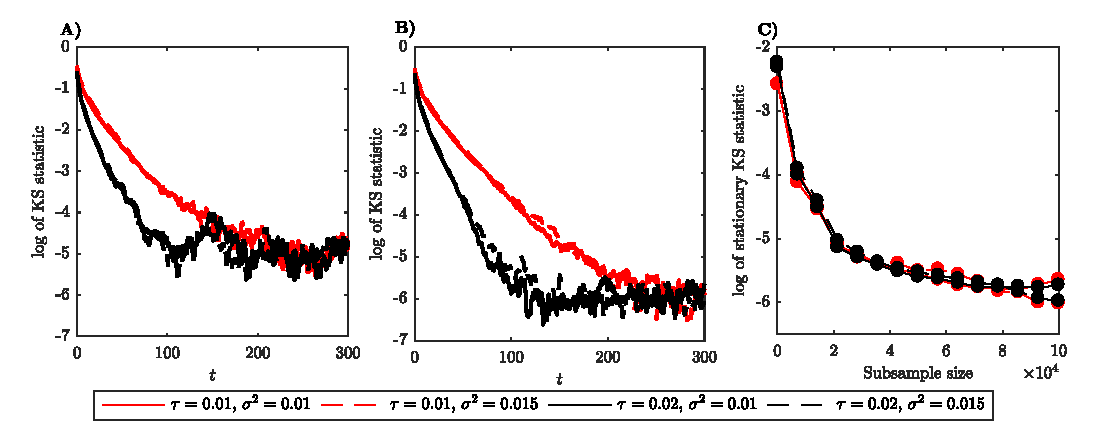
\includegraphics[width=1.0\textwidth]{figs/fig_mixing_time_rgbm.eps}
\caption{\textbf{Relaxation time in RGBM.} \textbf{A)} Total variational distance as a function of time for a realization of an RGBM process with a subsample size of $10^2$ for different noise amplitudes and reallocation parameters. \textbf{B)} Same as \textbf{A)}, only with a subsample size of $10^3$ people. \textbf{C)} The stationary total variational distance as a function of the subsample size for various $\sigma^2$ and $\tau$. In the simulations $N = 10^5$ people.\label{fig:rgbm-mixing-time}}
\end{figure}


\end{document}

%% THIS SECTION IS OUT OF THE DOCUMENT AND IT IS NOT NEEDED FOR NOW
\section{Derivation of IEE in RGBM}

As a measure, the intragenerational earnings elasticity is determined by the dynamics of the log of (rescaled) wealth $z = \log(y)$. Using Ito calculus, we can recover the following equation for the dynamics of $z$,
\begin{align*}
    d z &= \tau \bigg( \exp(-z) - \frac{2\tau + \sigma^2}{2 \tau} \bigg) dt + \sigma dW.
\end{align*}
The stationary distribution of the process can be found by using the transformation law of probabilities, 
\begin{align}
    P_z(z) &= P_y\big(\exp(z)\big) \exp(z).
\end{align}
The first and second moment of this distribution are
\begin{align}
\langle z \rangle &= -\psi(\theta) + \log(\theta - 1), \\
\langle z^2 \rangle &= \psi^{(1)}(\theta) + \bigg( \psi^{(1)}(\theta) - \log(\theta-1)\bigg)^2.
\end{align}
See \citet{DutreDebosscher1977,Debosscher1990} for the derivation of the transitory PDF of both $y$ and $z$.
